%! Tex program = xelatex
\documentclass{article}

%\usepackage[UTF8]{ctex}
\usepackage{amsmath,amssymb}
\usepackage{ntheorem}
\usepackage[letterpaper,top=2cm,bottom=2cm,left=3cm,right=3cm,marginparwidth=1.75cm]{geometry}%table package
%Table
\usepackage{multirow,booktabs}
\usepackage{makecell}
%字体颜色
\usepackage{color}
\usepackage[dvipsnames]{xcolor}  % 更全的色系
%代码
\usepackage[OT1]{fontenc}
\usepackage[framed,numbered,autolinebreaks,useliterate]{/Users/anye_zhenhaoyu/Desktop/Latex/mcode}
\usepackage{listings}
\usepackage{algorithm}
\usepackage{algorithmic}
%插图
\usepackage{graphicx}
%改变item格式
\usepackage{enumerate}
%物理
\usepackage{physics}
%extra arrows
\usepackage{extarrows}

\def\RR{\mathbb{R}}
\def\ZZ{\mathbb{Z}}
\def\EE{\mathbb{E}}

\def\Trsp#1{#1^{\mathcal{T}}}

\def\bw{\boldsymbol{\omega}}
\def\ba{\boldsymbol{a}}
\def\bb{\boldsymbol{b}}
\def\bc{\boldsymbol{c}}
\def\bd{\boldsymbol{d}}
\def\bt{\boldsymbol{t}}
\def\bx{\boldsymbol{x}}
\def\by{\boldsymbol{y}}
\def\bz{\boldsymbol{z}}
\def\vvert{\vert\vert}
\def\bA{\boldsymbol{A}}
\def\bB{\boldsymbol{B}}
\def\bC{\boldsymbol{C}}
\def\bE{\boldsymbol{E}}
\def\bO{\boldsymbol{O}}
\def\bX{\boldsymbol{X}}
\def\bY{\boldsymbol{Y}}

\def\Esolve{\textcolor{blue}{Solve: }}
\def\Eproof{\textcolor{blue}{Proof: }}

\def\suminf#1{\sum_{#1=-\infty}^{+\infty}}

\newtheorem{lemma}{Lemma}
\newtheorem{proof}{Proof}
\newtheorem*{theorem}{Theorem}


\begin{document}
\title{Homework 5}
\author{Zhen}
\maketitle

\section*{Problem 1}
$$
\bx^*=\mathop{\arg\min}_{\bx\in\bar{B}}f(x)=\frac{1}{2}\norm{\bx-\bx_0}^2
$$
\Eproof
$$
\nabla f=\bx-\bx_0
$$
Also, the optimal point is unique because $\nabla^2f>0$.
\\
Considering that: $\forall\bx\in\bar{B}$,
$$
\begin{aligned}
	\nabla f(\frac{\bx_0}{\norm{\bx_0}})^{\mathcal{T}}
	(\bx-\frac{\bx_0}{\norm{\bx_0}})
	&=
	(\frac{\bx_0}{\norm{\bx_0}}-\bx_0)^{\mathcal{T}}
	(\bx-\frac{\bx_0}{\norm{\bx_0}})
	\\
	&=
	(1-\frac{1}{\norm{\bx_0}})
	(\norm{\bx_0}-\bx_0^{\mathcal{T}}\bx)
	\\
	&\ge
	(1-\frac{1}{\norm{\bx_0}})
	(\norm{\bx_0}-\norm{\bx_0}\times\norm{\bx})
	\\
	&\ge
	0
\end{aligned}
$$
By first-order optimality condition, we conclude that $\bx^*=\frac{\bx_0}{\norm{\bx_0}}$.
\section*{Problem 2}
The graph of question (a),(b) and (c) are as follows.
\begin{figure}[h]
	\centering
	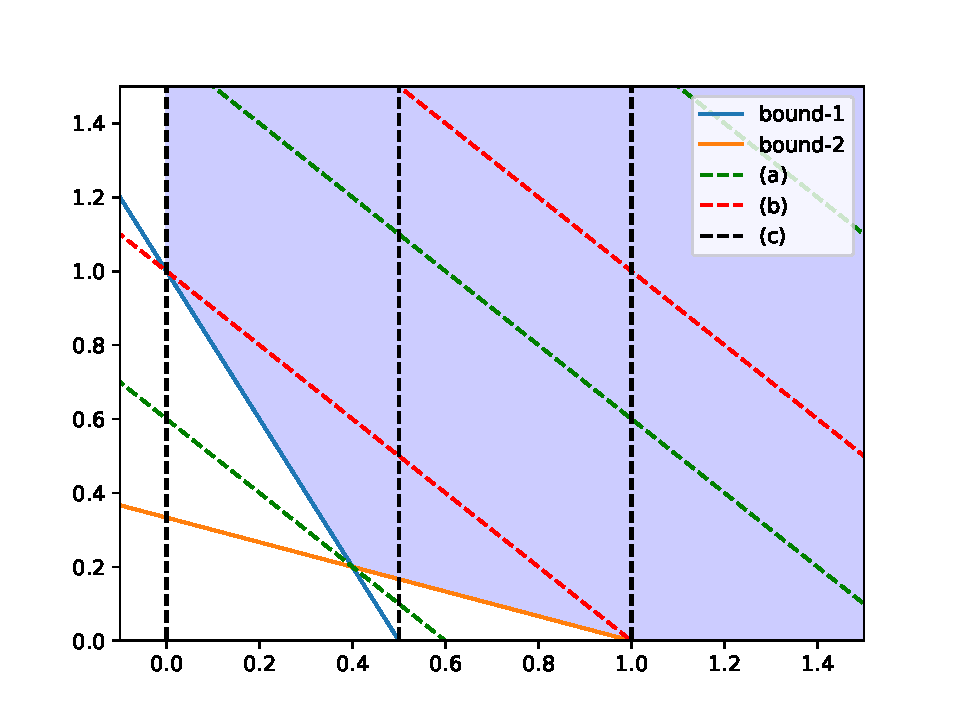
\includegraphics[width=0.5\textwidth]{P2.pdf}
\end{figure}

In the graph, the light blue area means the feasible set. And the series of dotted lines demonstrate the counter of function $f$.
\\
So the solution for each questions is:\\
(a) $x_1=0.4,x_2=0.2,f=0.6$\\
(a) $x_1=-\infty,x_2=-\infty,f=+\infty$, which means no optimal point.\\
(a) $x_1=0,x_2=C(\ge1),f=0$

\newpage
The code is at ``P2.py''.
\begin{figure}[h]
	\centering
	\includegraphics[width=0.5\textwidth]{p2-Rslt.png}
\end{figure}


\section*{Problem 3}

\begin{enumerate}[(a)]
	\item 
		$\bA \stackrel{def}{=}
		\qty(\ba_1,\ba_2,\dots,\ba_m)^\mathcal{T},
		\bb \stackrel{def}{=}
		\qty(b_1,b_2,\dots,b_m)^{\mathcal{T}},
		\bx \stackrel{def}{=}
		\qty(x_1,x_2,\dots,x_m)^{\mathcal{T}}
		$.
		Then we obtain
		$$
		\norm{\bA\bx-\bb}_1
		=
		\sum_{i=1}^m\abs{\ba_i^\mathcal{T}\bx-b_i}
		$$
		Also, 
		$$
		\begin{aligned}
			\norm{\bx}_\infty\le1
			\iff
			&\max_i{\abs{x_i}}\le1
			\\
			\iff
			&\abs{x_i}\le1,\ (\forall i\in\qty{1,\dots,n})
			\\
			\iff
			&\bx\le\boldsymbol{1}\land-\bx\le\boldsymbol{1}
		\end{aligned}
		$$
		Introducing $\bt=(t_1,t_2,\dots,t_n)^{\mathcal{T}}$, we could reformulate the optimization problem as:
		$$
			\begin{aligned}
			\min_{\bx,\bt}\ \ 
			&\boldsymbol{1}_m^{\mathcal{T}}\bt
			\\
			\mbox{\textbf{s.t.}}\ \ 
			&-\boldsymbol{1}_n\le\bx\le\boldsymbol{1}_n
			\\
			&\forall i\in\qty{1,2,\dots,m}:
			-t_i\le\ba_i^{\mathcal{T}}\bx-b_i\le t_i
		\end{aligned}
		$$
		Rewrite the afformentioned optimal problem ($\bw=\mqty[\bx\\\bt]$):
		$$
			\begin{aligned}
				\min_{\bw}\ \ 
			&\mqty[\boldsymbol{0}_n \\ \boldsymbol{1}_m]^{\mathcal{T}}\bw
			\\
			\\
			\mbox{\textbf{s.t.}}\ \ 
			&
			\mqty[
				\bE_{n\times n} & \bO_{n\times m} \\
				-\bE_{n\times n} & \bO_{n\times m} \\
				\bA & -\bE_{m\times m} \\
				-\bA & -\bE_{m\times m} 
			]\bw
			\le
			\mqty[
				\boldsymbol{1}_n \\
				\boldsymbol{1}_n \\
				\bb \\
				-\bb
			]
		\end{aligned}
		$$
	\item
		The code is at ``P3b.py''.
		\begin{figure}[h]
		\centering
		\includegraphics[width=0.5\textwidth]{p3b.png}
		\end{figure}
	\newpage
	\item
		The code is at ``P3c.py''.
		\begin{figure}[h]
		\centering
		\includegraphics[width=0.5\textwidth]{p3c.png}
		\end{figure}
\end{enumerate}


\section*{Problem 4}
\begin{enumerate}[(a)]
	\item 
		$f(\bw)\stackrel{def}{=}\norm{\bX\bw-\by}_2^2$ and $\bw^*=\mathop{\arg\min}_{\bw}f(\bw)$. Considering that:
		$$
		\begin{aligned}
			&f(\bw)=\Trsp{\bw}\Trsp{\bX}\bX\bw
			-2\Trsp{\by}\bX\bw+\Trsp{\by}\by
			\\
			&\nabla f(\bw)=2\Trsp{\bX}\bX\bw
			-2\Trsp{\bX}\by
		\end{aligned}
		$$
		By the fact that $\nabla f(\bw^*)=0$, we have
		$$
		\begin{aligned}
			\bw^*&=\qty(\Trsp{\bX}\bX)^{-1}\Trsp{\bX}\by=\mqty[1.5\\2]
		\end{aligned}
		$$
	\item
		The code is at ``P4b.py''.
		\begin{figure}[h]
			\centering
			\includegraphics[width=0.5\textwidth]{p4b.png}
		\end{figure}
		\\
		When $t=1$, the solution is \textbf{NOT} the same as that of (a) and has a zero component.
		\\
		When $t=10$, the solution is the same as that of (a) and does not contain a zero component.

	\item
		The code is at ``P4c.py''.
		\begin{figure}[h]
			\centering
			\includegraphics[width=0.5\textwidth]{p4c.png}
		\end{figure}
		\\
		When $t=1$, the solution is \textbf{NOT} the same as that of (a) and does not has a zero component.
		\\
		When $t=10$, the solution is the same as that of (a) and does not contain a zero component.

\end{enumerate}

\end{document}

